% THIS IS SIGPROC-SP.TEX - VERSION 3.1
% WORKS WITH V3.2SP OF ACM_PROC_ARTICLE-SP.CLS
% APRIL 2009
%
% It is an example file showing how to use the 'acm_proc_article-sp.cls' V3.2SP
% LaTeX2e document class file for Conference Proceedings submissions.
% ----------------------------------------------------------------------------------------------------------------
% This .tex file (and associated .cls V3.2SP) *DOES NOT* produce:
%       1) The Permission Statement
%       2) The Conference (location) Info information
%       3) The Copyright Line with ACM data
%       4) Page numbering
% ---------------------------------------------------------------------------------------------------------------
% It is an example which *does* use the .bib file (from which the .bbl file
% is produced).
% REMEMBER HOWEVER: After having produced the .bbl file,
% and prior to final submission,
% you need to 'insert'  your .bbl file into your source .tex file so as to provide
% ONE 'self-contained' source file.
%
% Questions regarding SIGS should be sent to
% Adrienne Griscti ---> griscti@acm.org
%
% Questions/suggestions regarding the guidelines, .tex and .cls files, etc. to
% Gerald Murray ---> murray@hq.acm.org
%
% For tracking purposes - this is V3.1SP - APRIL 2009

\documentclass{acm_proc_article-sp}

\usepackage[ngerman]{babel}
\usepackage[utf8]{inputenc}
\usepackage{tikz}
\usepackage{float}
\usepackage{rotating}


\begin{document}

%\title{Complex Network Analysis mit R}
%\subtitle{Kategorien bei Artikeln eines wissenschaftlichen Fachsgebiets in der Wikipedia}
\title{Untersuchung der Kategorisierung von Artikeln von wissenschaftliche Forschungsgebieten in der Wikipedia}

\numberofauthors{1} 
\author{
% 1st. author
\alignauthor
	First Author\\
	\affaddr{Universität}\\
	\email{peterr@github.com}
}

\maketitle
\begin{abstract}
In dieser Arbeit soll die Struktur der Kategorien und dazugehörige gemeinsame Vergabe in Artikel untersucht werden. Die Vegabe soll anhand einer wissenschaftlichen Oberkategorie durchgeführt werden. Versucht wird hierbei weitere Forschunggebiete aus dem Oberthema zu erkennen und zu extrahieren. Weiter sollen wichtige Kategorien aufgefunden werden, die die kleineren Forschungsgebiete vernetzen, sowie mit Forschungsgebieten aus anderen wissenschaftlichen Diziplinen verbinden.
\end{abstract}

\section{Einführung}
In der Wikipedia werden den Artikel Kategorien zugeordnet. Ein Artikel kann in beliebig viele Kategorien gelistet werden. Der Aufbau der Kategorien ist hierachisch. Jedoch die Kategorisierung von Artikel bilden kein hierachisches Netzwerk, da ein Artikel z.B. in zwei von einander getrennten Wissenschaftgebieten eingeordnet werden können. Die Kategorievergabe ist in der Wikipedia nicht standardisiert und auch nicht automatisiert. Kategorien werden manuell von den Nutzern vergeben und können fehlerhaft sein. Mithilfe eines Netzwerks aus den Kategorien der Artikel sollen folgende Fragen untersucht werden. 

\subsection{Fragestellung}
Bildet die Kategorisierung der Artikel in der Wikipedia, die Forschungsgebiete der Wissenschaft ab? Dass heißt bilden sich Gruppen von Kategorien, die wissenschaftlich nahe verwandt sind? Ebenso wird interessant ist die Frage, welche Kategorien wissenschaftliche Felder verknüpfen bzw. welche davon zentral für die Teilgebiete der Forschung sind.

\section{Datensatz}
Der Datensatz für die Analyse der Kategorien von wissenschaftlichen Fachgebieten wurde über die API der englischen Wikipedia gewonnen. Es wurde die Kategorie \textbf{machine Learning} als beispielhaftes Themengebiet ausgewählt, um die Analyse durchzuführen. Bei unserer Analyse wurde nur die Artikel berücksichtigt, die direkt unter der Kategorie als Seiten aufgelistet werden.

\subsection{Aufbau des Netzwerks}
Die Kategorien der Artikel bilden in unserem Netzwerk bilden die Knoten und haben außer dem Namen der Kategorie keine weiteren Eigenschaften. Die Kanten zwischen den Kategorien beschreiben die Bezeihung, dass beide Kategorien zusammen einem Artikel zugeordnet wurden. 
\begin{figure}[H]
\centering
\begin{tikzpicture}[scale=2]
\tikzstyle{every node}=[sloped,draw,shape=rectangle];
\node            (a) at (0,0)  {Kategorie A};
\node[draw=none] (art1) at (1,-0.2) {in Artikel 1};
\node[draw=none] (art2) at (1,0.45) {in Artikel 2};
\node[draw=none] (art3) at (0.05,-0.5) {in Artikel 1};
\node[draw=none] (art4) at (1.95,-0.5) {in Artikel 2};
\node            (b) at (2,0)  {Kategorie B };
\node            (c) at (1,-1) {Kategorie C };
\draw[-, bend right] (a) edge (b); 
\draw[-, bend left] (a) edge (b);
\draw[-] (a) edge (c);
\draw[-] (b) edge (c);
\end{tikzpicture}
\caption{Struktur des Netzwerkes}
\end{figure}
Die Kanten sind ungerichtet, da beide Kategorien in einem Artikel immer zusammen verwendet werden. Zwischen zweiKnoten können keine, eine oder mehr Kanten existieren. Mehr als eine Kanten zwischen zwei Knoten, existieren nur, wenn die beiden Kategorien in mehreren Artikel zusammen verwendet werden.

\section{Eigenschaften des Netzwerkes}
Das hier vorliegende Netzwerk, dass die Kategorisierung von Artikel der Kategorie maschinelles Lernen darstellt, existieren alle Kanten nur einmal. Das heißt jede der Kombinationen von Kategorien wurde nur einmal vergeben.
Für die weitere Analyse wurde die Kategorie Machine Learning aus dem Graph entfernt, da diese in jedem Artikel auftritt. Dieser Umstand ist dem Verfahren zum Erzeugen des Netzwerkes geschuldet. Das Netzwerk hat $116$ Kategorien und $199$ Kanten. Es gibt also $199$ Kombinationen von Kategorien, die auf den Seiten der Oberkategorie maschinelles Lernen verwendet wurden. Hierbei sind jedoch auch Kategorien, die Wikipedia-spezifisch sind, z.B. stubs. Diese wurden bei der Analyse nicht weiter berücksichtigt.
\newpage
\subsection{Basismetriken}
\begin{figure}[H]
\centering
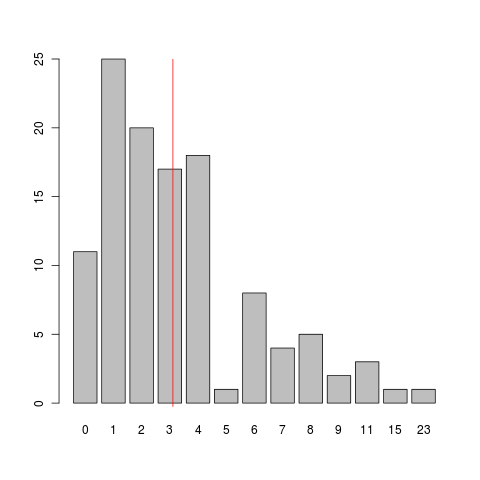
\includegraphics[scale=0.35]{../visualization/degree_hist.png}
\caption{Gradverteilung des Netzwerks}
\label{fig:degree}
\end{figure}
\subsubsection{Degree}
Die durschnittliche Gradanzahl der Knoten beträgt $3.4$ und der maximale Grad eines Knoten ist $23$. Der Knoten mit dem maximalen Grad ist die Kategorie \textbf{Data Mining}. Außerdem haben $11$ Knoten keine Kanten. Sie sind also von den anderen Kategorien isoliert. Die Verteilung der Knotengrade, als auch der Mittelwert(rot), ist in Abbildung \ref{fig:degree} zu sehen. In Tabelle \ref{tab:degree} sind die Kategorien mit den größten Degree aufgelistet
\begin{table}[H]
\centering
\begin{tabular}{lr}
\hline
Kategorie & degree \\ 
\hline
Data mining & 23 \\ 
Classification algorithms & 11 \\ 
Image processing & 11 \\ 
Information retrieval & 15 \\ 
Numerical analysis & 9 \\ 
\hline
\end{tabular}
\caption{Kategorien mit höchstem degree}
\label{tab:degree}
\end{table}
\subsubsection{Dichte}
Die Dichte des Netzwerkes beträgt $2.9\%$. Es handelt sich also um ein Netzwerk, dass angesichts der maximal möglichen Kanten, nur sehr dünn verbunden ist.
\subsubsection{Transitivität}
Der globale Clusterkoeffizient des Netzwerkes hat einen Wert von $0.53$. Dasbedeutet eine Kategorie hat mit einer $53$-prozentigen Wahrscheinlichkeit eine Verbindung zu einer anderen Kategorie.
\subsubsection{betweenness}
Die Betweenness gibt die Wichtigkeit als Zentrale Knoten eines Netzwerkes an. Wieder zeigt sich deutlich, dass die Kategorie Data Mining eine zentrale Rolle spielt unter den Kategorien im Bereich des maschinellen Lernensi(zu sehen in Tabelle \ref{tab:close}. Aber auch die Kategorien Information retrieval und Data analysis haben einen hohenbetweenness-Wert.
\begin{table}[H]
\centering
\begin{tabular}{lr}
\hline
Kategorie & betweenness \\ 
\hline
Data mining & 1349.83 \\ 
Information retrieval & 437.53 \\ 
Data analysis & 330.98 \\ 
Artificial intelligence conferences & 305.15 \\ 
Image processing & 192.00 \\ 
\hline
\end{tabular}
\caption{Kategorien mit höchster betweenness}
\label{tab:close}
\end{table}

\subsubsection{closeness}
Bei den closeness-Werten ist ein Interpretation schwierig, da die Variation der Werte nur sehr gering ist. Das liegt daran es in dem Netzwerk isolierte Komponenten und Knoten gibt, wodurch die Berechnung der closeness verzerrt wird. Trotzdem sind in der folgenden Tabelle \ref{tab:close} die Kategorien mit den größten closeness-Werten aufgelistet.
\begin{table}[H]
\centering
\begin{tabular}{lr}
\hline
Kategorie & closeness \\ 
\hline
Data mining & 0.02 \\ 
Data analysis & 0.02 \\ 
Cluster analysis & 0.02 \\ 
Artificial intelligence conferences & 0.02 \\ 
Information retrieval & 0.02 \\ 
\hline
\end{tabular}
\caption{Kategorien mit der höchsten closeness}
\end{table}
\subsubsection{shortest paths}
Die durschnittliche Länge der kürzesten Pfade in unserem Netzwerk beträgt $3.15$(In der Abbildung \ref{fig:paths} rot eingezeichnet). Die meisten kürzesten Pfade haben die Länge 2. Die meisten Kategorien sind also über sehr wenige andere Knoten miteinander verbunden, dass lässt darauf schließen, dass es einige sehr wichtige Knoten für das Netzwer gibt. 
\begin{figure}[H]
\centering
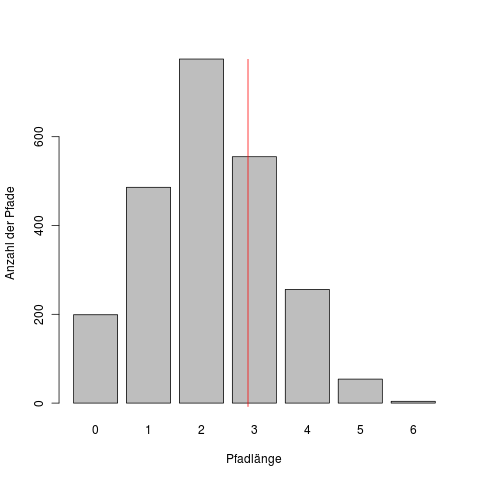
\includegraphics[scale=0.55]{../visualization/shortest_path_hist.png}
\caption{Verteilung der Pfadlängen}
\label{fig:paths}
\end{figure}
\newpage
\section{Analyse}
\subsection{Cluster}
Bei der Clusteranalyse zeigt sich, dass insgesamt 24 Cluster in unserem Netzwerk existieren. Davon haben jedoch 11 nur die größe 1. Für die weitere Untersuchungen werden die Cluster der Größe nicht betrachtet, dass heißt wir haben 13 Cluster mit mindestens 2 Kategorien.
Der größte Cluster beinhaltet 68 Kategorien, also mehr als die Hälfte aller Kategorien in unserem Netzwerk.
In diesem Cluster befinden sich auch alle bisher in dieser Arbeit aufgetretenen Kategorien, wie Data Mining oder Information Retrieval. In Abbildung \ref{fig:clusters} sind die Cluster des Netzwerks grafisch dargestellt.
\begin{figure}[H]
\centering
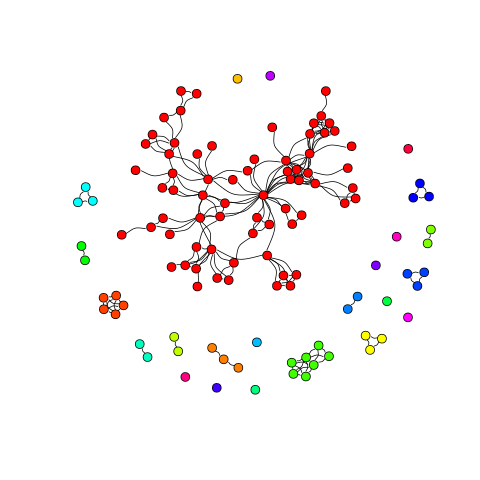
\includegraphics[scale=0.55]{../visualization/ml_cluster_graph.png}
\caption{Cluster im Netzwerk}
\label{fig:clusters}
\end{figure}
Der auf der Abbildung grüne Cluster beinhaltet Kategorien für Publikationen aus dem Bereich des maschinellen Lernens. Dazu gehören z.B. Computer Science Journals oder Open access Journals. Auch der drittgrößte Cluster mit 5 Kategorien beinhaltet nur Kategorien die auf Bildungsinstitute verweisen und werden deshalb entfernt. Für die folgenden Analyse der Communities des Netzwerks konzentrieren wir uns auf das größte Cluster mit den 68 Kategorien.
\subsection{Communities}
Um die Communities in unseren Netzwerk zu entdecken haben wir bereits gesehen, dass nur die Suche nach Communities in dem größten Cluster sinnvoll ist. Dieanderen Clustern sind zu klein, damit sich dort Communities herrausbilden können und sind genausogroß wie die Cluster.

Es zeigt sich, dass Kategorien, die eine hohen betweenness-Wert haben wichte Verbindungsknoten zwischen die Communities bilden. Die Kategorie Information Retrival verbindet z.B. die schwarzen und hellblaun Communities. Aber auch die Kategorie Data Mining zeigt sich als Verbindung zwischen Communities in diesem Cluster. Sie ist der Übergang zwischen grüner und hellbauer Community.

In Abbildung \ref{fig:communities} ist anhand der Farben zu sehen, dass sich 6 Communties bilden. Die grüne Community bildet ein Art Zentrum für die anderen Communties, die sich um die grüne Community gruppieren.
\begin{figure}[H]
\centering
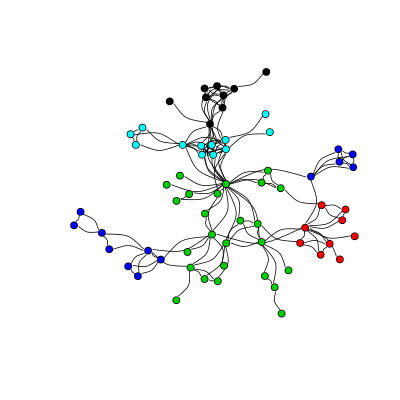
\includegraphics[scale=0.6]{../visualization/ml_community_graph.png}
\caption{Communities im größten Cluster des Netzwerks}
\label{fig:communities}
\end{figure}
\section{Ergebnisse}
Die Analyse zeigt, dass sich Themengruppen im Netzwerk der vergebenen Kategorien finden lassen. Sowohl bei der Clusteranalyse, als auch bei der Suche nach Communities, lassen Themenbereichen finden. Teilweise ist die Abgrenzung nicht eindeutig gegeben. Bei den kleineren Clustern geht die Einteilung noch ganz gut. Das zweitgrößte Cluster kann auf Kategorien für wissenschaftliche Publikationen beschränkt werden und das drittgrößte auf Bildungsinstitute.
Kleinere Cluster sind wenig aussagekräftig, was unter anderem an zu wenigen Daten für das Netzwerk liegen mag. Alle Cluster, die kleiner sind als des größten sind, bilden wiederum eine Community. Auch bei sogennanten Themen kann bei den kleineren Clustern keine Aussage getroffen werden, da sie dadurch zu sehr von der großen Zahl der Kategorien abgeschnitten ist, um weitere Erkenntnisse zu gewinnen.

Interessanter scheint hierbei der größte Cluster mit 68 Knoten zu seien. DieCommunity-Analyse hat gezeigt, dass sich dort 6 Communties bilden. Aber auch hier sind die Themen nicht immer ganz leicht einzugrenzen. Die kleineren Communties, die sich um die große grüne Community bilden sind nicht immer zu gebrauchen. Die beiden dunkelblauen Communities lassen sich noch beschreiben.
Eine Community beschäftigt sich mit neuronalen Netzwerken und Algorithmen und beinhaltet ebenfalls die zugrundeliegende Neurowissenschaften als Kategorie. Die andere Community beinhaltet Kategorien, die sich mit Entscheidungsfindung und Verfahren beschäftigt. Dazu gehören die Kategorien Decision theory oder Cognitive science, die wieder naha verwand zu den Neurowissenschaften sind, jedoch ist im Netzwerk keine konkrete Beziehung zwischen beiden Communities zu erkennen.

Die größte Community lässt sich jedoch nicht so leicht zusammenfassen. Sie enthält Kategorien, wie statistical models, decision trees, aber auch Natural language processing. Natürlich gehören alle diese Kategorien zur Oberkategorie machine learning. Eine weitere Differenzierung ist mit dieser Community jedoch nicht möglich. Hierfür ist wohl auch das kleine Netzwerk verantwortlich. Die Cluster - und Communtiyanalyse war also nicht sehr ergiebig.

Was sich gezeigt hat ist die Verkünpfung von grundlegenden Katgorien des machinellen Lernens mit den Wissenschaften aus denen sie abgeleitet wurden. Als Beispiele sind hier zu nennen die Verbindung zwischen den Kategorien Neural networks und Neuro science oder auch Bayesian statistics mit der Kategorie decision threory. Insgesamt sind sehr viele Kategorien aus dem Bereich der Stochastik vertreten. Die dazugehörigen Bereiche können jedoch nur schwer in unserem Netzwerk unterteilt werden.

Darüberhinaus lassen sich wichtige Kategorien aus dem Bereich des maschinellen Lernens sehr gut erkennen. Die wichtigen Themen scheinen Data mining, Information retrival, Cluster und Data analysis zu sein. Es zeigt sich also, das zumindest häufige Anwendungsgebiete relativ einfach anhand unseres Netzwerkes erkennen lassen. Anwendungsgebiete können dadurch identifziert werden, wenn sie mit viele verschiedene Kategorien einer Oberkategorien verbunden sind. Eine Erklärung dafür könnte sein, dass sich diese Anwendungsgebiete bei viele Erkenntnissen und Ergebnissen anderer Kategorien bedienen. 

\section{Related Work}
Es gibt einige Arbeiten, die sich mit der Kategoriesierung in der Wikipedia beschäftigen. Es konnten aber keine Publikationen gefunden werden, die sich nur mit der Struktur der gemeinsamen Vergabe von Kategorien beschäftigen. Einige Arbeiten beschäftigen sich mit der Klassifizierung von Texten anhand der Klassifizierung in der Wikipedia, wie etwa \cite{Weale_utilizingwikipedia}. Andere Arbeiten verwenden die Struktur der Kategorien in der Wikipedia als Hilfsmittel für die Verarbeitung von natürlicher Sprache \cite{tubiblio32662}.
\section{Zusammenfassung und Ausblick}
Im Laufe der Arbeit hat sich gezeigt, dass der Datensatz für ein wirklich aussagekräftiges Ergebnis zu klein ist. Deswegen wäre die Einbeziehungen von direkten Unterkategorien der Kategorie machine learning sinnvoll gewesen.

Auch wenn bei der Erstellung des Datensatzes darauf geachtet wurde, dass keine Wikipedia-spezifischen Kategorien mit aufgenommmen werden, gab es Kategorien, die das Ergebnis leicht verändert haben. Diese Kategorien befanden waren vor allem zugenannte stub-Kategorien, also Kategorien für Artikel, die weiter ausgearbeitet werden sollen. Andererseits könnten solche Kategorien auch für eine qualitativere Analyse verwendet werden. Bei Stubs könnte nicht nur der Inhalt verbesserungsbedürftig sein, sondern auch die Kategorisierung, dass heißt solche Artikel könnten ausgeschlossen werden.

Wie bereits im Abschnitt Related Work angesprochen, gibt es eine Vielzahl von Einsatzmöglichkeiten, die der Analyse der Kategorisierung in der Wikipedia zugrunde liegen.  \cite{*}
\bibliographystyle{abbrv}
\bibliography{report}
\newpage
\begin{figure}
\centering
\begin{sideways}
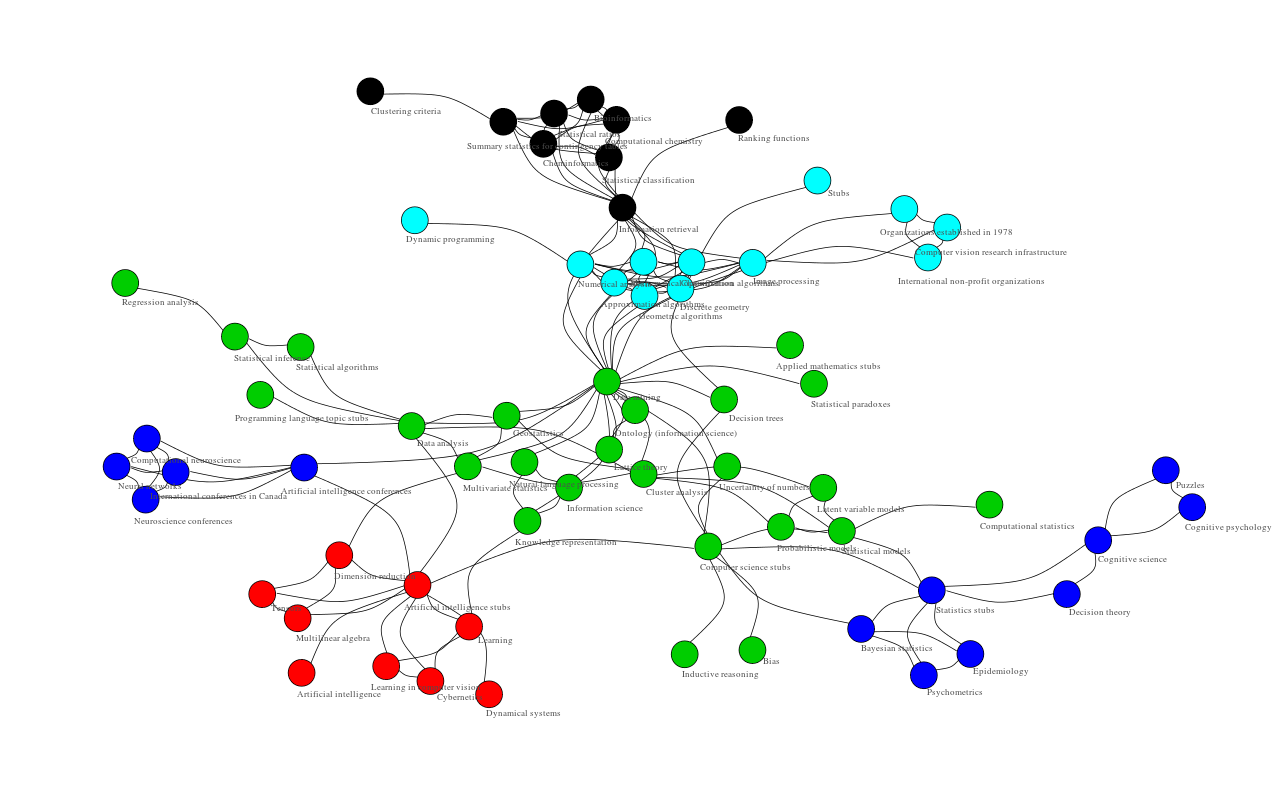
\includegraphics[scale=0.5]{../visualization/ml_graph_big.png}
\end{sideways}
\caption{Communities des gesamten Netzwerks}
\label{fig:big}
\end{figure}
\end{document}  % This is where a 'short' article might terminate
